\chapter{Introduction}
\section{Background}
%%% discuss huge volume of contents and why content valuation is needed 
\subsection{Inforamtion Overload}
In the age of information explosion, people are overwhelmed by the redundant content and data. As shown in the figure \ref{fig:data}, volume of data has experienced exponential growth recently and this trend will continue in the next few years.

\vspace{5pt}
\begin{figure}
\centering
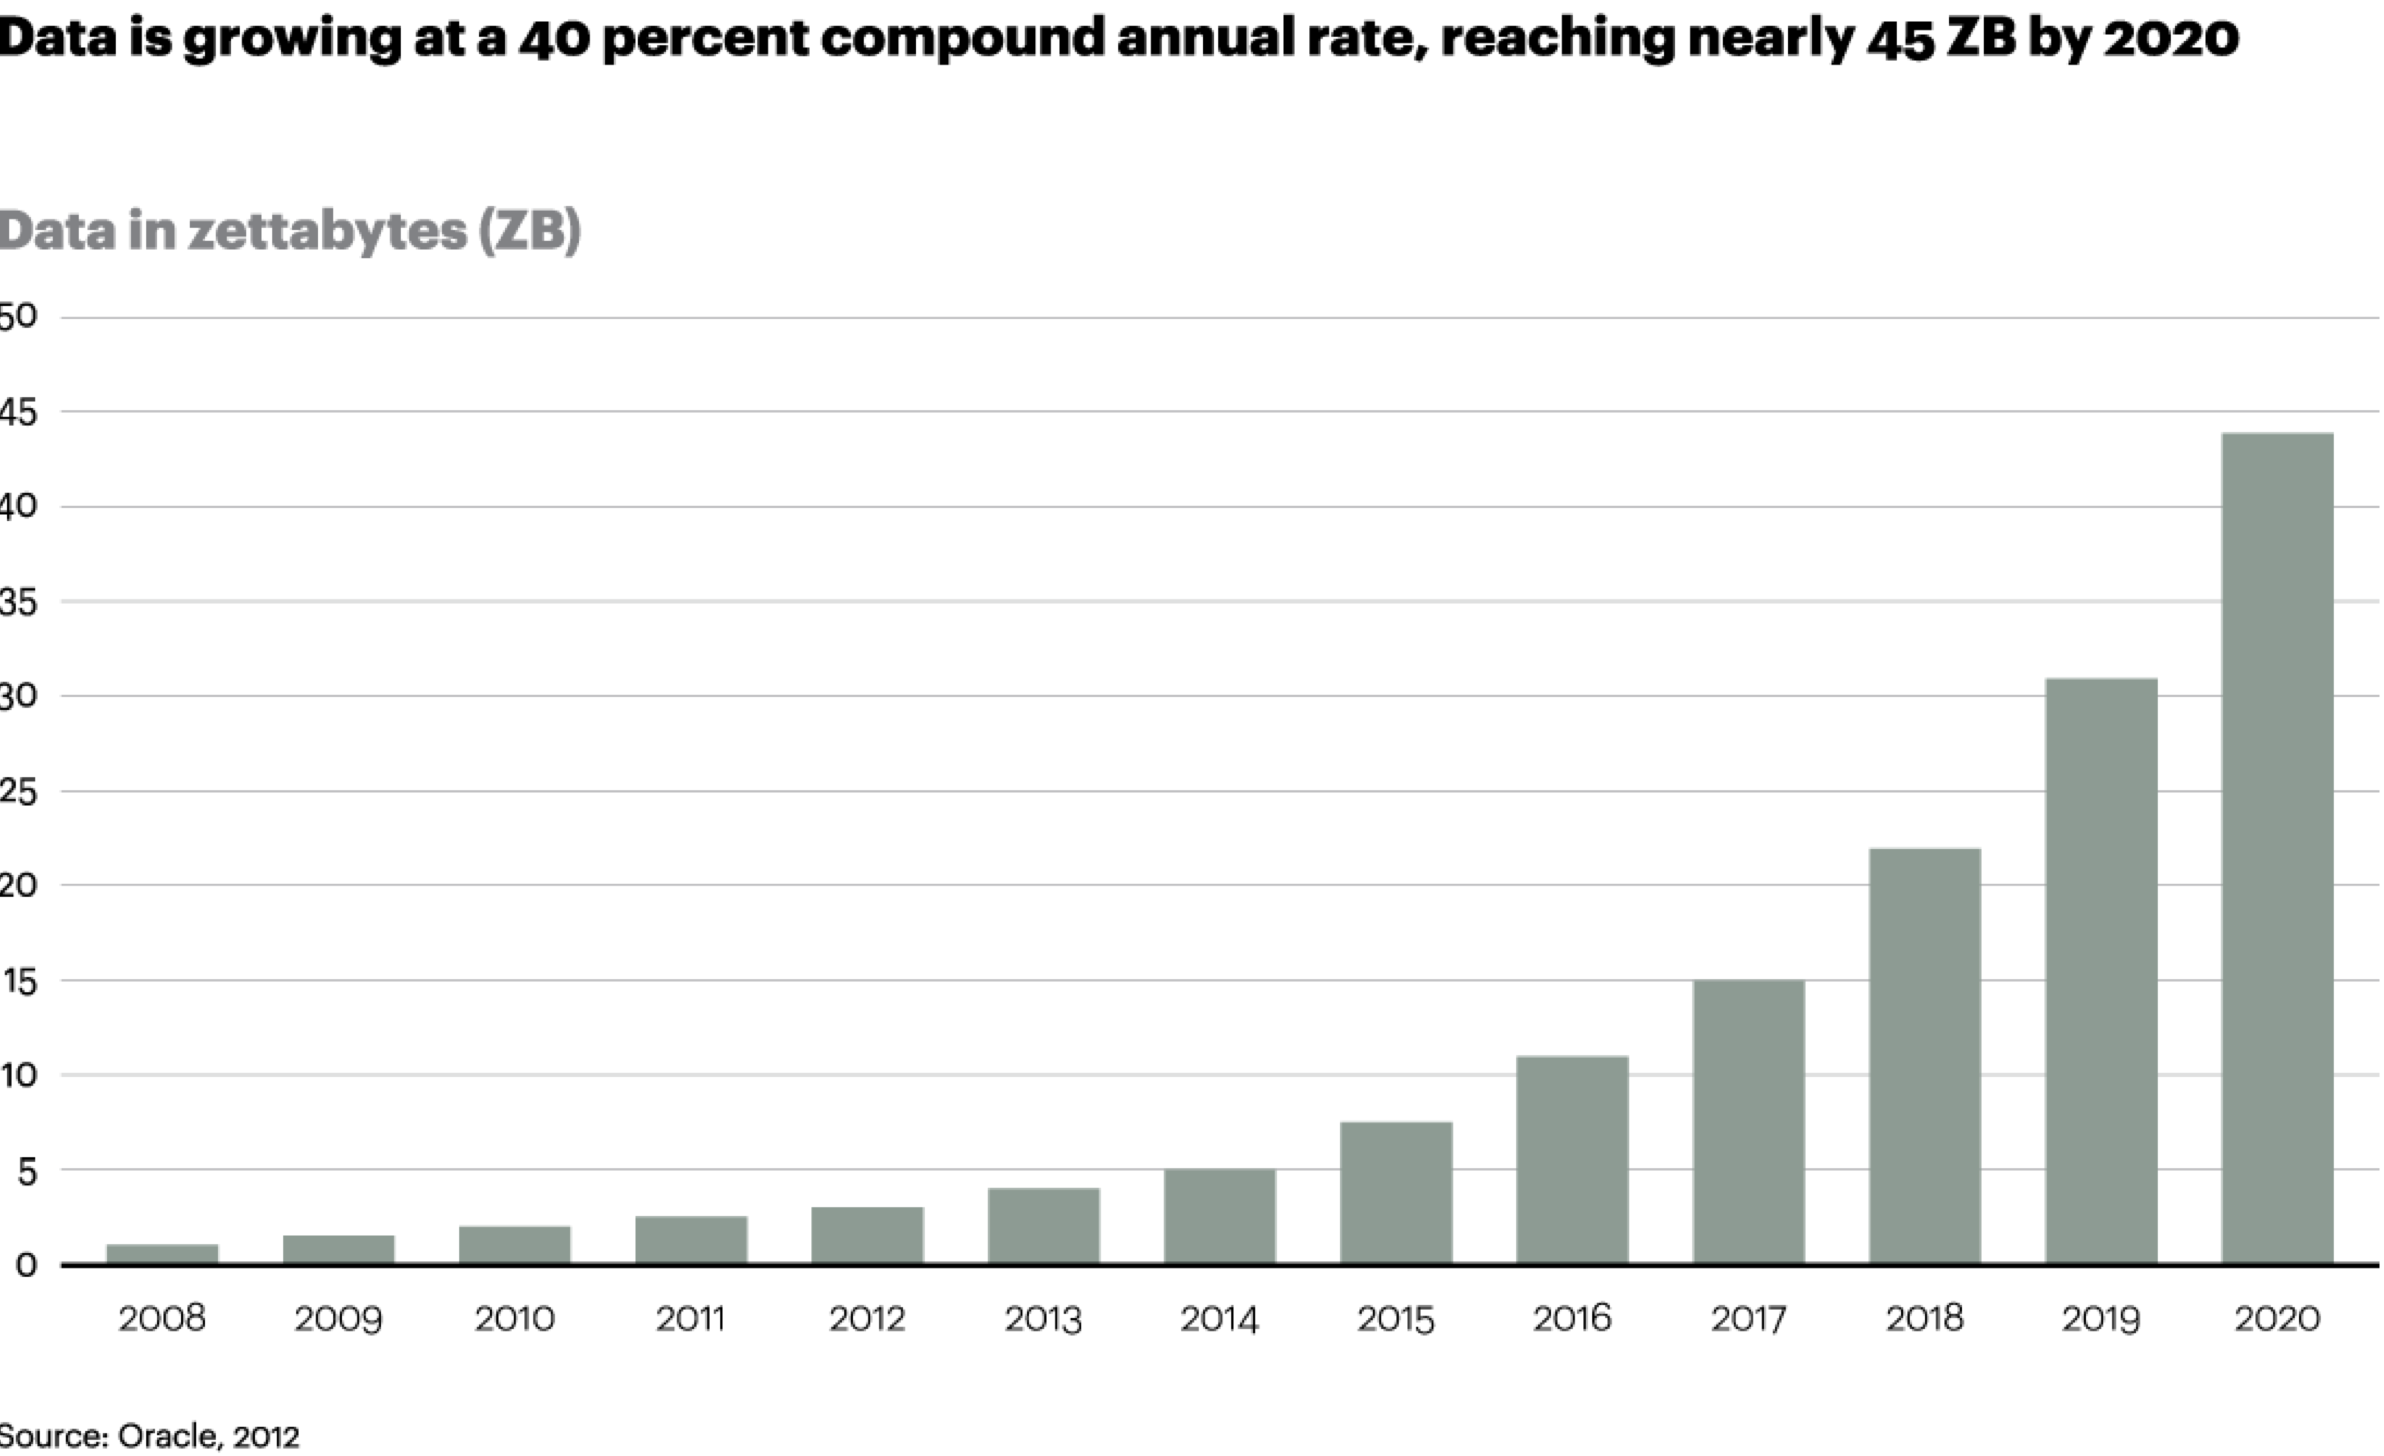
\includegraphics[width=\linewidth]{data_grow.png}
\caption{Exponential Growth of Data Information}
\label{fig:data}
\end{figure}

%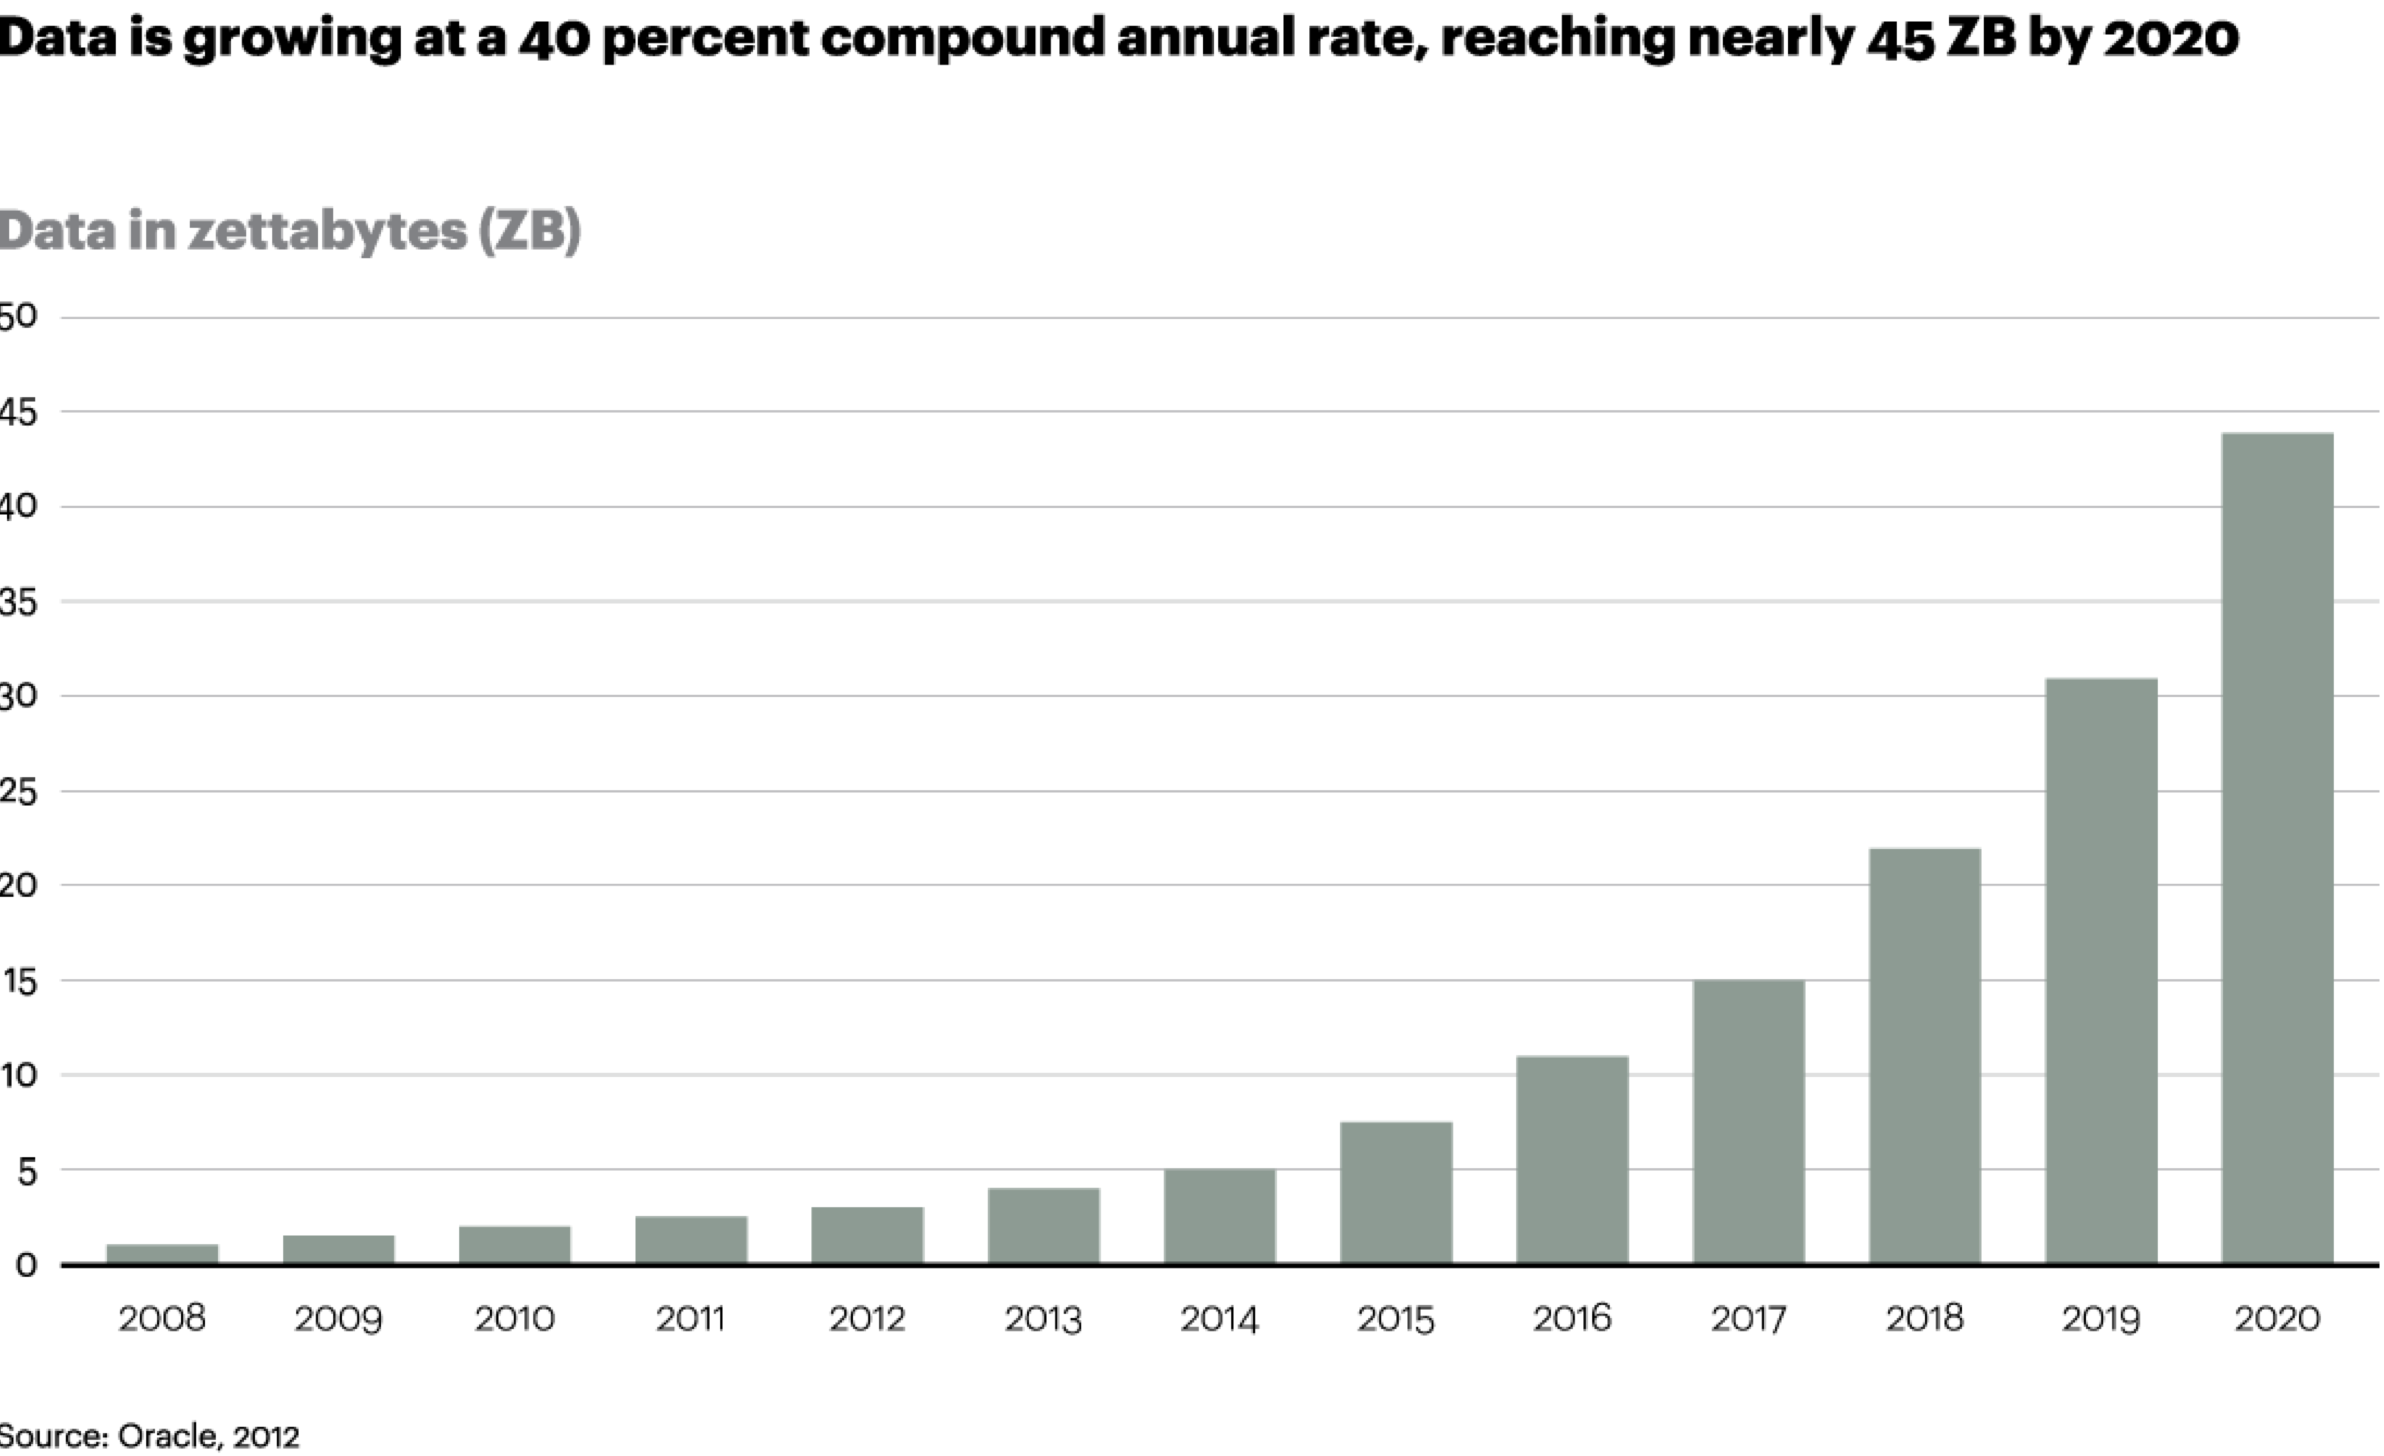
\includegraphics[width=\linewidth]{data_grow.png}

With the rapid growth of Internet, more information are generated and shared across the world with ever-faster speed, which causes several issues:
\begin{itemize}
\item \textbf{Low Quality Issue}: Many content creators generate large volume of contents without paying attention to quality, therefore, adding more superficial, distracting, or eye-catching contents with low quality. As such, audience can easily ignore high-value contents due to the interference of low-quality contents. 
\item \textbf{Copyright Issue}: Several content creators simply copy others' contents from the Internet and publish to their audience with/without modification, which is actually plagiarism and infringement. In current environment, it is really hard to trace back the original copyright ownership of one piece of content. 

\end{itemize}
Therefore, it becomes urgent but extremely challenging to identify those high-value contents from vast amount of information and reward original owners with less effort. 

\subsection{Problems of Centralized Platforms}
Existing user-generated-content communities, such as Facebook, Youtube, Wikipedia and Twitter, usually have their own centralized authorities, which monitor and control the operation of the entire community. They have several drawbacks as following:

\begin{itemize}
\item \textbf{Biased Content Judgment}: those authorities have all privileges, such as promoting, recommending, and deleting contents. In this scenario, only those authorities have the rights to promote high-value contents, so they may generate biased judgment according to their own criteria. The regular audience in those communities have no opportunity to promote their valued contents.

\item \textbf{Centralized Content Storage}: In those communities all user-generated-contents are stored in the centralized server or data center, which may cause service interrupt or outage when the centralized storage fails.  Much worse, the contents may be damaged or even lost and no longer available to be accessed. 

\item \textbf{Unfair Distribution of Benefits}: Usually the communities takes most income distribution from advertisement or audience payment, while content creators receive a very small piece or even no benefit at all.  

\end{itemize}
Those drawbacks make existing communities less attractive to contents creators and audience, because they are note motivated to create and promote high-value contents. 


\section{Why \emph{U Network} ?}
The solution to those issues of existing user-generated-content platforms is \emph{U Network}, which has following functionality:
\begin{enumerate}
    
    \item \textbf{discovering high-quality content}: By leveraging a decentralized prediction market to assess the quality of a content, \emph{U Network} provides an efficient way to find out high-quality information and avoids prejudice.    
    \item \textbf{reasonably distributing benefit}:  \emph{U Network} allocates monetized token rewards to the platform contributors with the help of content pricing mechanism. The contributors includes both content creator and any regular users who promote valuable contents with up-votes.
    
    \item \textbf{decentralizing content storage}: \emph{U Network} will support IPFS protocol (InterPlanetary File System\cite{ipfs}), a persistent internet file transfer protocol, or Genaro Network, a fault tolerant, tamper-resistant, permanent storage protocol. These decentralized storage solutions not only improve the reliability of data integrity but also guarantee the availability of contents using redundant copies across distributed server nodes.       
\end{enumerate}

\subsection{Mission of \emph{U Network}}
The mission of \emph{U Network} is to build a user-generated-contents community based on blockchain technology, which is a content-value based prediction market driven by quality and value of contents. This platform has following advantages compared with existing communities:
\begin{itemize}
\item content creators are motivated to generate more high-quality contents, because they receive monetized token rewards when their contents receive up-votes from more audience. 
\item all participants can receive token rewards when they promote high-value contents with up-vote. This is because contents with more up-votes will be assigned higher priority and become much easier to be accessed by audience.
\item Each up-vote in  \emph{U Network} costs certain amount of tokens, which is similar to \emph{Gas} in Ethereum network and represents the price of up-vote that users need to pay. This cost of up-vote becomes the income source of token rewards that distributed to contributors, and prevents malicious users gaming the up-vote mechanism for rewards. 
\end{itemize}

As such, more valuable contents will be generated in this community and all participants are motivated to discover and promote those high-value contents. 

From the theoretical point view, this motivation model is derived from ``efficient-market hypothesis'' \cite{efficient}.  The efficient-market was first introduced by Bachelier, who first recognized the efficiency of the market in selecting information. In short, the discounting of past, present, and future events have their reflections in the current market price. His theory assumes that investors in the market are rational and are looking for their self interest in maximizing their own profits, and each individual has an independent analysis of the value of a content. Therefore, it becomes feasible to leverage the wisdom of all participants in this community to set a price for each content, where the price serves as an accurate prediction of the true value.  

\subsection{Content-Value based Prediction Market}
The key component of  \emph{U Network} and affiliated communities is the prediction market. In principle, prediction market\cite{prediction} is a platform where people trades the outcome of events. In this prediction market, people receive profit if their predictions proved to be correct. The reward distribution follows a simple but fair and robust principle: reward is transferred from inaccurate predictors to accurate ones. Knowing this rule, people would try their best effort to gather more information and make their best predictions to receive the rewards.

The construction of the  \emph{U Network} prediction market follows the similar idea. Users can up vote to promote a piece of content with the cost of some \emph{U Network} tokens. If other audience think the current prediction underestimate the value of contents, they may up vote with more tokens. In this way, the cost of up-vote for high-quality contents keeps increasing, and accordingly the user who promote this content with up-vote can gain monetized token reward. 

To sum up,  \emph{U Network} will be constructed to be a content-value driven platform powered by blockchain. It is revolutionary to use the content-value prediction market to motivate all participants to discover and promote high-quality contents using token incentives. Therefore, it becomes much easier to discover high-quality contents with great value in the user-generated-content community.






